% Options for packages loaded elsewhere
\PassOptionsToPackage{unicode}{hyperref}
\PassOptionsToPackage{hyphens}{url}
%
\documentclass[
]{article}
\usepackage{amsmath,amssymb}
\usepackage{lmodern}
\usepackage{iftex}
\ifPDFTeX
  \usepackage[T1]{fontenc}
  \usepackage[utf8]{inputenc}
  \usepackage{textcomp} % provide euro and other symbols
\else % if luatex or xetex
  \usepackage{unicode-math}
  \defaultfontfeatures{Scale=MatchLowercase}
  \defaultfontfeatures[\rmfamily]{Ligatures=TeX,Scale=1}
\fi
% Use upquote if available, for straight quotes in verbatim environments
\IfFileExists{upquote.sty}{\usepackage{upquote}}{}
\IfFileExists{microtype.sty}{% use microtype if available
  \usepackage[]{microtype}
  \UseMicrotypeSet[protrusion]{basicmath} % disable protrusion for tt fonts
}{}
\makeatletter
\@ifundefined{KOMAClassName}{% if non-KOMA class
  \IfFileExists{parskip.sty}{%
    \usepackage{parskip}
  }{% else
    \setlength{\parindent}{0pt}
    \setlength{\parskip}{6pt plus 2pt minus 1pt}}
}{% if KOMA class
  \KOMAoptions{parskip=half}}
\makeatother
\usepackage{xcolor}
\usepackage[margin=1in]{geometry}
\usepackage{graphicx}
\makeatletter
\def\maxwidth{\ifdim\Gin@nat@width>\linewidth\linewidth\else\Gin@nat@width\fi}
\def\maxheight{\ifdim\Gin@nat@height>\textheight\textheight\else\Gin@nat@height\fi}
\makeatother
% Scale images if necessary, so that they will not overflow the page
% margins by default, and it is still possible to overwrite the defaults
% using explicit options in \includegraphics[width, height, ...]{}
\setkeys{Gin}{width=\maxwidth,height=\maxheight,keepaspectratio}
% Set default figure placement to htbp
\makeatletter
\def\fps@figure{htbp}
\makeatother
\setlength{\emergencystretch}{3em} % prevent overfull lines
\providecommand{\tightlist}{%
  \setlength{\itemsep}{0pt}\setlength{\parskip}{0pt}}
\setcounter{secnumdepth}{-\maxdimen} % remove section numbering
\usepackage{wrapfig}
\usepackage{booktabs}
\usepackage{longtable}
\usepackage{array}
\usepackage{multirow}
\usepackage{wrapfig}
\usepackage{float}
\usepackage{colortbl}
\usepackage{pdflscape}
\usepackage{tabu}
\usepackage{threeparttable}
\usepackage{threeparttablex}
\usepackage[normalem]{ulem}
\usepackage{makecell}
\usepackage{xcolor}
\usepackage{siunitx}
\newcolumntype{d}{S[input-symbols = ()]}
\ifLuaTeX
  \usepackage{selnolig}  % disable illegal ligatures
\fi
\IfFileExists{bookmark.sty}{\usepackage{bookmark}}{\usepackage{hyperref}}
\IfFileExists{xurl.sty}{\usepackage{xurl}}{} % add URL line breaks if available
\urlstyle{same} % disable monospaced font for URLs
\hypersetup{
  pdftitle={Covid-19 Wastewater Flagging Method Optimization},
  pdfauthor={Marlin Lee, Abe Megahed, Kyllan Wunder; University of Wisconsin Data Science Institute - October 2022},
  hidelinks,
  pdfcreator={LaTeX via pandoc}}

\title{Covid-19 Wastewater Flagging Method Optimization}
\author{Marlin Lee, Abe Megahed, Kyllan Wunder \and University of
Wisconsin Data Science Institute - October 2022}
\date{}

\begin{document}
\maketitle

\hypertarget{introduction}{%
\subsection{Introduction:}\label{introduction}}

In this analysis, we perform a comparative analysis of various
wastewater flagging techniques with the goals of (1) making the
wastewater flags match the case analysis flags and (2) reducing false
positives in the reported wastewater flags. As the adoption of at-home
tests increases and case reporting decreases, wastewater becomes a more
important metric for determining true case numbers. Accurate flagging
methods are critical for policymakers to make better-informed decisions
based on predicted changes in cases.

\noindent

\begin{wrapfigure}[14]{R}{0.6\textwidth}
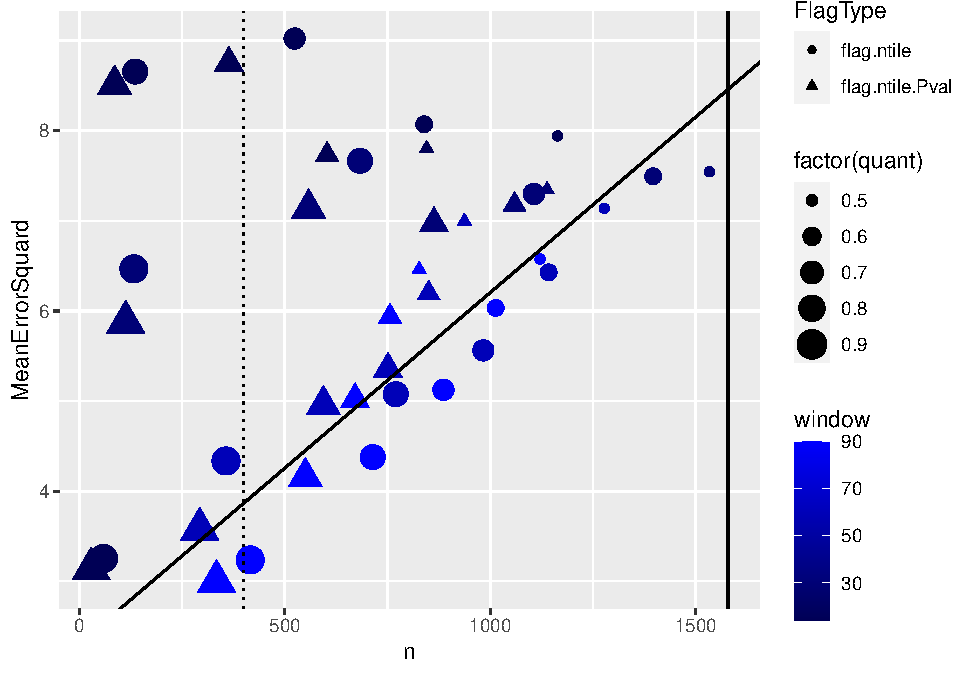
\includegraphics{optimising_flagging_method_files/figure-latex/unnamed-chunk-2-1} \caption{The angled line is a linear regression line based on the 60 and 90-day intervals. The vertical lines represent the total number of case flags (1578) and the proportion of wastewater samples to wastewater flags if they had the same ratio as cases to case flags (389)}\label{fig:unnamed-chunk-2}
\end{wrapfigure}

\hypertarget{flagging-methods}{%
\subsection{Flagging Methods}\label{flagging-methods}}

The DHS has created flagging methods based on wastewater measurements
and aims to supplement existing case flagging metrics. The wastewater
method uses a 5-day regression to see if the predicted change is above
100\%. If so, it checks if the last 3-day average is larger than the K
day Q quantile (where K and Q are customizable parameters). Then if both
are true, it is labeled as a flag.ntile. If the Linear regression has a
p-value below .3, it is labeled as a flag.ntile.Pval. We explored five
quantile values (.5, .6, .7, .8,..9) and four window values (14, 30, 60,
90 days) for a total of 40 ways to flag\\
models.

\hypertarget{graph-explanation}{%
\subsection{Graph explanation}\label{graph-explanation}}

The graph shows a distinct linear relationship between the variance and
the number of flags produced (denoted on the graph by the diagonal
regression line). This relationship makes it possible to balance the
number of flags against the allowable variance or to determine the
expected variance for a particular number of flags. We calculate the
squared distance each wastewater flag is from the nearest case flag to
find the optimal combination. On investigation, it becomes clear the
major issue with current options is the number of flags reported. As
quantile size increases, the data fits this trend more, and with a
smaller quantile size, the mean squared error (MSE) is much more varied.

\hypertarget{matching-wastewater-flags-to-case-flags}{%
\subsection{Matching wastewater flags to case
flags}\label{matching-wastewater-flags-to-case-flags}}

The case flag method has 1578 flags, so the chosen wastewater method
should have an equal amount. None of the methods create that many flags;
most produce multiple times less due to the lower frequency of
wastewater sampling. This means we could expect proportionally fewer
flags; this is shown by a dashed line where you might expect the number
of flags if it was proportional.

\begin{wraptable}{r}{0pt}
\centering
\begin{tabular}[t]{lcc}
\toprule
  & Full Model & Scaled Down Model\\
\midrule
(Intercept) & \num{5.1644} & \num{2.3083}\\
 & P-val = \num{0.0000} & P-val = \num{0.0000}\\
n & \num{0.0015} & \num{0.0039}\\
 & P-val = \num{0.0287} & P-val = \num{0.0000}\\
\midrule
Num.Obs. & \num{40} & \num{20}\\
R2 & \num{0.120} & \num{0.797}\\
RMSE & \num{1.56} & \num{0.53}\\
\bottomrule
\end{tabular}
\end{wraptable}

\hypertarget{linear-model-lm-explanation}{%
\subsection{Linear Model (LM)
explanation}\label{linear-model-lm-explanation}}

We created two linear models to explain the relationship between the
number of points and the error. First, we used the whole data set and
found minimal relation. Second, we excluded the 14 and 30 day windows
and got a very successful linear model shown in the previous plot.

\hypertarget{conclusion}{%
\subsection{Conclusion}\label{conclusion}}

We found no one best model because there is an inherent tradeoff between
MSE and the number of flags created. However, a great candidate is the
90 day window 90\% percentile flags which are around the correct number
of adjusted flags and have the lowest MSE score.

\end{document}
